\section{Background}

In this section I'll provide a self-contained explanation of Yao's Garbled Circuits.

Multi-party computation, or MPC, is a kind of cryptographic protocol where several people send some messages back and forth. The point of an MPC protocol is to compute the output of some function on private inputs held by each party, but without those parties needing to share their inputs. If you could trust someone to do the computation and keep everyone's inputs secret, then the calculation would be easy. MPC removes the need to trust other parties, though.

Multi-party computation can refer to any kind of computation involving any number of parties (greater than one). In this paper, I focus on one protocol under this umbrella, Yao's Garbled Circuits, which performs computations between two parties by evaluating a Boolean circuit.

\subsection{Boolean Circuits}

\begin{figure}[t]
	\centering
	\begin{tikzpicture}
		\node[xor port] (xor)  at (0, 0){};
		\node[and port] (andA) at (3, .7){};
		\node[and port] (andB) at (3,-.7){};
		\draw (andA.in 1)  -- ++(-5, 0)
		      (andB.in 2)  -- ++(-5, 0)
		      (xor.in 1)   -| ++(-1, .7) node [below right] {A}
		      (xor.in 2)   -| ++(-1,-.7) node [above right] {B}
		      (andA.in 2)  -|  (xor.out) node [      right] {C}
		      (andB.in 1)  -|  (xor.out)
		      (andA.out) node [above] {D} -- ++(1, 0)
		      (andB.out) node [above] {E} -- ++(1, 0);
	\end{tikzpicture}
	\caption{An example Boolean circuit with one XOR gate and two AND gates. The inputs wires are on the left and the outputs are on the right.}%
	\label{fig:circuit}
\end{figure}

A Boolean circuit is a collection of logic gates connected together by wires. Each wire receives a label, with the computation's inputs assigned to the wires on the left. Each gate then compares the labels on its inputs to the gate's own lookup table to determine what label to assign to its output wire on the right. The contents of the lookup table determine how the gate behaves, and we give names to several common sets of table contents. For example, if 0 and 1 are the possible labels for each wire, and correspond to False and True respectively, then Tab.~\ref{tab:truth-table} shows an XOR gate and two AND gates, right-to-left.

Circuits like these can compute any mathematical expression. (For usage in MPC, circuits can't have loops, so any looping algorithm will need its loops unrolled to be represented as a circuit.)

\begin{table}[ht]
	\centering
	\begin{tabular}{cc|c   cc   cc|c   cc   cc|c}
		A & B & C   &&&   A & C & D   &&&   C & B & E \\
		\cmidrule{1-3}    \cmidrule{6-8}    \cmidrule{11-13}
		0 & 0 & 0   &&&   0 & 0 & 0   &&&   0 & 0 & 0 \\
		0 & 1 & 1   &&&   0 & 1 & 0   &&&   0 & 1 & 0 \\
		1 & 0 & 1   &&&   1 & 0 & 0   &&&   1 & 0 & 0 \\
		1 & 1 & 0   &&&   1 & 1 & 1   &&&   1 & 1 & 1 \\
	\end{tabular}
	\caption{Truth tables for the gates in Fig.~\ref{fig:circuit}. Each column is labeled to match a wire and each row matches an input combination to an output value.}%
	\label{tab:truth-table}
\end{table}

\comment{What it means to evaluate a circuit}

\comment{One block of SHA256 takes 130000 gates}

\subsection{Garbled Circuits}
Boolean operations are represented by tables, but these tables don't have to map Trues and Falses, and in fact the outputs don't have to match the inputs at all. For example, consider \comment{truth table with letters instead of true/false}. Naturally, one can still evaluate a circuit without knowing what the labels correspond to. This forms the basis for garbling.

Keys and boxes.

Abstract transformation by one party, computation in transformed space, first party provides info to transform back.

\subsection{Yao's Garbled Circuits}
This protocol was first described by Andrew Yao in 1986 at that year's IEEE Annual Symposium on Foundations in Computer Science. In the most basic terms, one party ``garbles'' the circuit by encrypting and transposing the inputs to each logic gate, then sends the stream of garbled gates to a second party, who evaluates the garbled circuit with their own private inputs while learning nothing about the garbler's inputs.

This presents an asymmetry in which one party must calculate each node of the circuit for all inputs and broadcast a high volume of information while the other party performs about half the work and only sends back data about the inputs and outputs. This asymmetry is similar to the current cloud-computing model, where servers in data centers perform difficult calculations while the client does minimal work to interpret the result.

There have been several improvements to Yao's original protocol since it was published. The most recent at the time of writing is called Half Gates\cite{HalfGates}, which reduces the data sent from the garbler to the evaluator by short-circuiting AND gates to encode either buffers or inverters depending on each party's known inputs to that gate.

\subsection{Improvements on the Protocol}
Yao's original protocol wasn't described very clearly, actually. In particular, how does the evaluator know which row of the table to decrypt? One solution is trial decryptions. The garbler chooses keys to end with a bunch of zeros, and the evaluator decrypts until they find the one that ends with zeros. This is really bad for performance. Also there are so many ciphertexts to send around and that just sucks. Thankfully, some smart people have found improvements to the original protocol that don't impact the security.

\subsubsection{Permute and Point}
Permute the table in a deterministic way so that the keys point to the entry they decrypt. You get no info about the other entries, so it doesn't break anything.

\subsubsection{Row Reduction}
Since you just hash and XOR, the garbler can choose what they're applying the XOR to. If they always choose the same ciphertext for the first entry, then there's no need to transmit it.

Requires hash function that lets you choose ciphertext via XOR. So it's XOR with hash for control.

\subsubsection{Free XOR}
You can pick wire labels such that using XOR on the labels means using XOR on the logical values they represent. This requires the garbler to keep track of a private delta.

\subsubsection{Beyond}
Half gates and gadget-wise optimizations. Also you can drop some security guarantees to make things much easier.

\subsection{The Hash Function}
For theoretical cryptography, it's fine to pick any hash function. It could be considered an implementation detail that we use AES. I care about implementation details a lot though, so I'm actually gonna talk about it.

Combine inputs into the message, and the key is actually fixed. Add key. Sub, shift, mix. Repeat. Sub and shift. Done.

\subsection{Field-Programmable Gate Arrays}
\textit{FPGA} stands for Field-Programmable Gate Array. It's a kind of chip that implements reconfigurable logic. My coprocessor design runs on an FPGA rather than going through the prohibitively expensive process of manufacturing a ``real'' single-purpose chip. The ``gate array'' part of the name means that the chip is made of a grid of general-purpose elements, shown in the zoomed-out view on the left above. This part of the chip is called the fabric.

The ``field-programmable'' part of the name means that these connections can be reconfigured on-the-fly after the chip has been manufactured and shipped. I used this reprogramming capability to test each iteration of my design. Zooming in, you can see diagonal wires representing a connection between the bus lines and components internal to each element. There are several types of elements distributed across the fabric, including elements specifically for input and output, clock signal generation, digital signal processing, RAM, and basic elements, which contain registers and configurable lookup tables.

\begin{figure}[ht]
	\centering
	\begin{tikzpicture}
		\node (image) {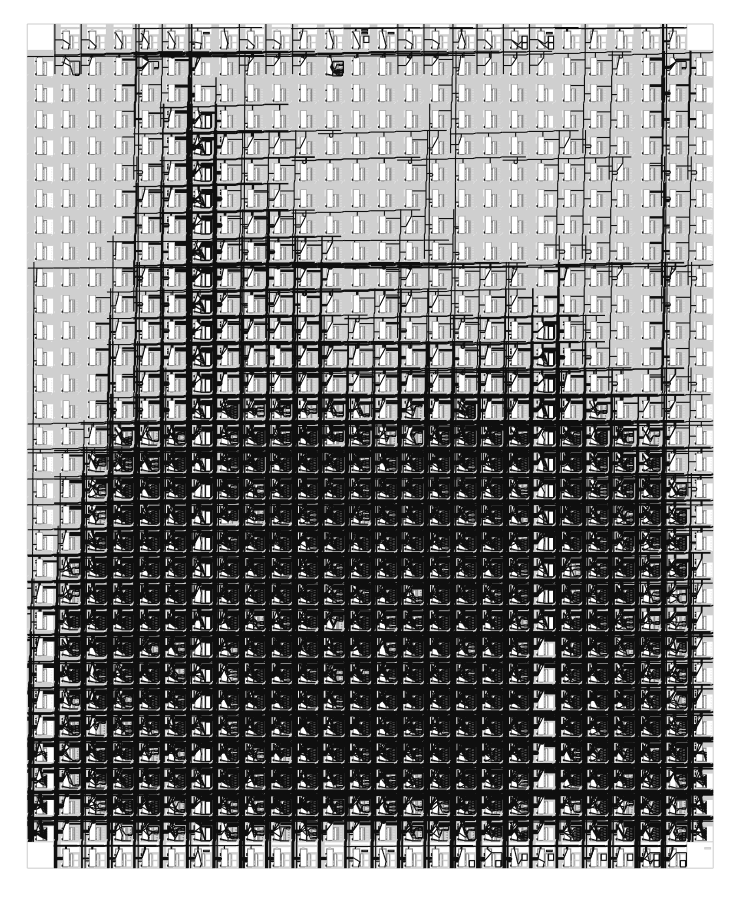
\includegraphics[width=.5\textwidth]{figures/fabric-full.png}};
		\draw[white, fill] (1,0) circle(3.5mm);
		\draw[white, line width=2mm]
			(130:3.1) ++(5,0) coordinate(top)
			(-130:3.1)++(5,0) coordinate(bottom)
			(130:.25)  ++(1,0) -- (top)
			(-130:.25) ++(1,0) -- (bottom);
		\begin{scope}[even odd rule]
			\draw[white, fill] (5,0) circle(3.2cm);
			\draw[black, ultra thick, fill=white] (5,0) circle(3.1cm);
			\clip (5,0) circle(3cm);
			\node (image) at (5,0) {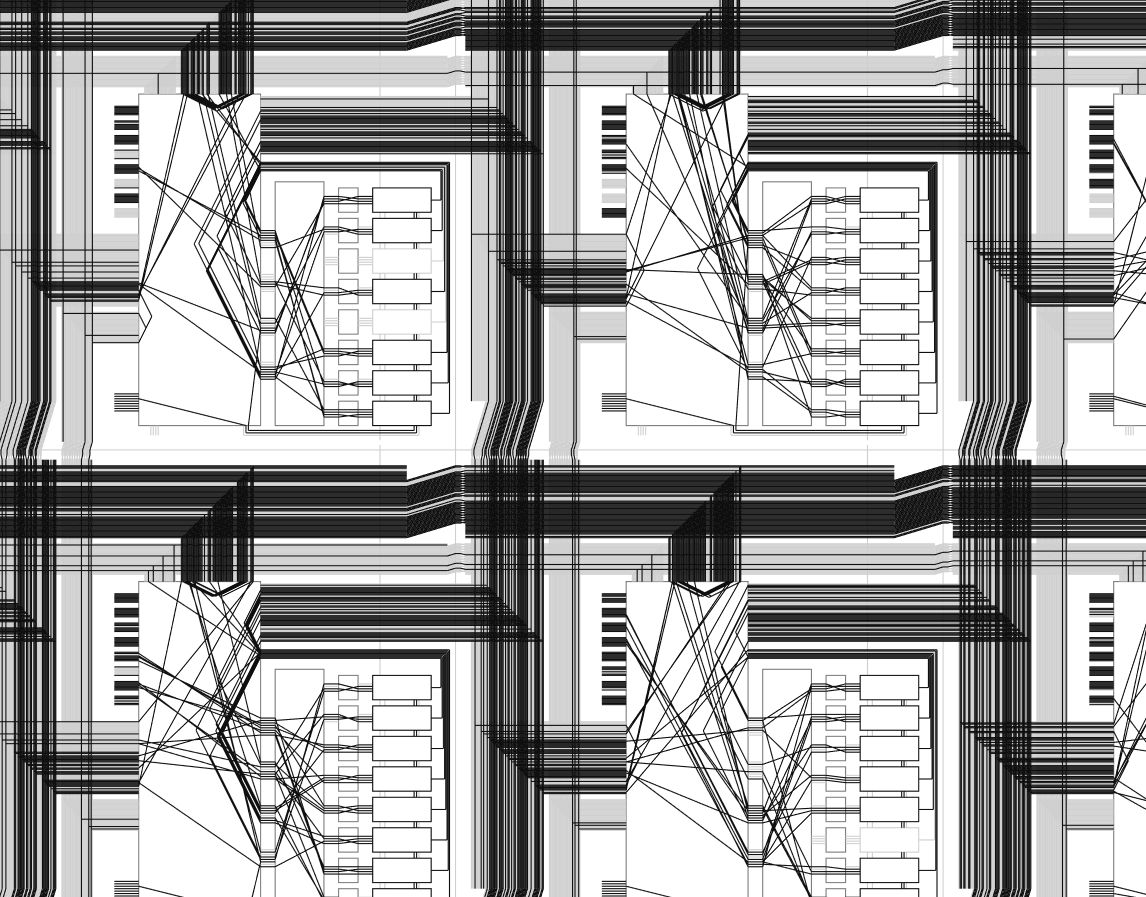
\includegraphics[height=6cm]{figures/fabric-zoom.png}};
		\end{scope}
		\draw[black, ultra thick]
			(130:3.1) ++(5,0) coordinate(top)
			(-130:3.1)++(5,0) coordinate(bottom)
			(130:.25)  ++(1,0) -- (top)
			(-130:.25) ++(1,0) -- (bottom);
		\draw[black, ultra thick, fill=white] (1,0) circle(2.5mm);
	\end{tikzpicture}
	\caption{Place and route output of my hardware design. The black wires represent the allocated interconnects. The zoomed portion shows the reconfigurable internals of several logic cells.}%
	\label{fig:pnr}
\end{figure}

Rather than code, a compiler, and an executable, the FPGA build toolchain has HDL, synthesis, place \& route, and the bitstream. HDL stands for ``hardware description language'' and it's the equivalent of ``code'' in software programming. I used the Verilog language to define the coprocessor, which is used to define state machines and combinational logic at the register-transfer level of abstraction. Synthesis is the process of turning this description into an abstract hardware definition. Place \& route is the process of placing circuit components onto elements of the FPGA fabric and routing connections between these components. Once the final FPGA configuration has been determined, it is serialized into a format that the FPGA chip can read to configure itself.\cite{IceStorm}

The FPGA configuration is volatile, so the bitstream must be sent to the chip each time the board turns on. The FPGA development board therefore includes a nonvolatile flash memory chip which stores the configuration bitstream and sends it to the FPGA when the board receives power.\cite{iCEBreaker}
